% This program is free software: you can redistribute it and/or modify
% it under the terms of the GNU AFFERO General Public License as published by
% the Free Software Foundation, either version 3 of the License, or
% (at your option) any later version.
%
% This program is distributed in the hope that it will be useful,
% but WITHOUT ANY WARRANTY; without even the implied warranty of
% MERCHANTABILITY or FITNESS FOR A PARTICULAR PURPOSE.  See the
% GNU General Public License for more details.
%
% You should have received a copy of the GNU AFFERO General Public License
% along with this program.  If not, see <https://www.gnu.org/licenses/>.
%
% Copyright (C) 2020 Mo Zhou <cdluminate@gmail.com>
%
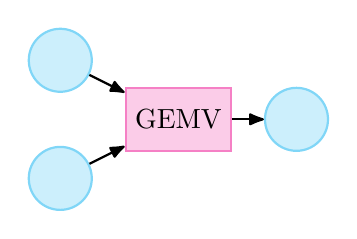
\begin{tikzpicture}[thick,minimum size=8mm]
	\usetikzlibrary{arrows.meta}
	\node (w) at (0,0) [circle,draw=cyan!50,fill=cyan!20] {$\mW$};
	\node (x) at (0,-1.5) [circle,draw=cyan!50,fill=cyan!20] {$\vx$};
	\node (gemv) at (1.5,-0.75) [rectangle,draw=magenta!50,fill=magenta!20] {GEMV};
	\node (y) at (3,-0.75) [circle,draw=cyan!50,fill=cyan!20] {$\vy$};
	\draw [-{Latex[round]}] (w) -- (gemv);
	\draw [-{Latex[round]}] (x) -- (gemv);
	\draw [-{Latex[round]}] (gemv) -- (y);
\end{tikzpicture}
